\documentclass{beamer}

\mode<presentation>

\usepackage[dutch]{babel}
%\usepackage{beamerthemesplit}
\usepackage{hyperref}

\usetheme{Berlin}
\useinnertheme{rounded}
\usecolortheme{rose}
\setbeamertemplate{navigation symbols}{} 
\title{Design patterns}
\author{W. Oele}
\date{\today}

\begin{document}
\frame{\titlepage}

\section{Design patterns}

\begin{frame}
\frametitle{Deze les}
\begin{itemize}
\item Factories
\item Het abstract factory patroon
\end{itemize}
\end{frame}


\begin{frame}
\frametitle{Factories: het probleem}
Code:
\begin{itemize}
\item houdt zich bezig met het cre\"eren van objecten
\item houdt zich bezig met het gebruiken van objecten
\end{itemize}
\end{frame}


\begin{frame}[fragile]
\frametitle{Voorbeeld}
\begin{verbatim}
public class Client
{
  public void maakenGebruik()
  {
     Auto a = new Auto();
     a.startMotor();
     a.rijNaar(Rotterdam);
     a.stopMotor();
  }
}
\end{verbatim}
\end{frame}


\begin{frame}
\frametitle{Factories}
Code die zich bezig houdt met het cre\"eren \emph{en} gebruiken van objecten:\pause
\begin{itemize}
\item client moet weten \emph{wat} er gecre\"eerd moet worden en \emph{hoe} het gecre\"eerde werkt.
\item high coupling
\item lastig te onderhouden
\item derhalve ongewenst
\end{itemize}
\end{frame}

\begin{frame}
\frametitle{Factories}
Uitdaging: Hoe het \emph{hoe} te scheiden van het \emph{wat}?\pause
\begin{itemize}
\item Client tegen verkoper: \emph{``Ik heb een schroevendraaier nodig\ldots''}
\item Verkoper: \emph{``Wat voor \'e\'en (groot/klein/kruiskop/torq/flat)?''}
\item Client: \emph{`` E\'en die werkt (kan mij wat schelen hoe ie werkt, als ie het maar doet)!'' }
\end{itemize}
\end{frame}

\begin{frame}
\frametitle{Factories: de client}
Het client object:
\begin{itemize}
\item wil op bepaalde momenten kunnen beschikken over objecten die iets doen.
\item is niet ge\"interesseerd in de interne werking van die objecten (het hoe).
\item is ge\"interesseerd in \emph{wat} en \emph{wanneer}.
\end{itemize}
\end{frame}

\begin{frame}
\frametitle{Factories}
De maker:
\begin{itemize}
\item houdt zich bezig met de vraag \emph{hoe} een object gemaakt moet worden.
\item is belast met varianten
\item is ge\"interesseerd in de eisen die aan een object worden gesteld en \emph{hoe} daaraan te voldoen.
\end{itemize}
\end{frame}

\begin{frame}
\frametitle{Ontwerpen}
Bij het ontwerpen:
\begin{itemize}
\item de \emph{hoe} vraag scheiden van de \emph{wat} vraag.
\item eerst nadenken over het wat:
  \begin{itemize}
  \item entiteiten:
  \item attributen
  \item operaties
  \item etc.
  \end{itemize}
\item daarna: nadenken over het \emph{hoe} en wie in je programma daar voor opdraait.
\end{itemize}
\end{frame}

\begin{frame}
\frametitle{Ontwerpen}
Algemeen:
\begin{itemize}
\item Denk eerst na over \emph{wat} je nodig hebt in je programma en aan welke eisen dat moet voldoen.
\item Denk \emph{daarna} pas na over wie dat gaat bouwen en hoe dat moet gebeuren.
\end{itemize}
\end{frame}

\begin{frame}
\frametitle{Factories}
\begin{itemize}
\item Client: \emph{``Ik heb een auto nodig!''}\pause
\item Verkoper: \emph{``Wat voor \'e\'en meneer?''}\pause
\item Client: \emph{``eentje met: ``}
  \begin{itemize}
  \item \emph{``vierwielaandrijving''}\pause
  \item \emph{``bestand tegen stof''}\pause
  \item \emph{``airco die aan en uit kan''}\pause
  \item \emph{``kooiconstructie''}\pause
  \item \emph{``motor die aan en uit kan''}
  \item \emph{``variabele snelheid''}
  \item \emph{``\ldots waarmee ik Parijs-Dakar kan rijden''}
  \end{itemize}
\end{itemize}
\end{frame}

\begin{frame}
\frametitle{Ontwerpen}
\begin{itemize}
\item Hoe een object te bouwen dat \emph{gegarandeerd} voldoet aan de eisen die een client object daaraan stelt?\pause
\item Antwoord:
\end{itemize}
\begin{center}
  \huge{INTERFACES}
\end{center}
Door na te denken over de interfaces, garandeer je bepaald gedrag bij de objecten die in je programma gebruikt worden. 
\end{frame}

\begin{frame}
\frametitle{Het abstract factory pattern}
\begin{itemize}
\item naam: het abstract factory pattern
\item doel: families van objecten aanbieden aan clients
\item hoe: gebruik van objecten scheiden van implementatie
\item gevolgen: nette boedelscheiding tussen wat/wanneer en hoe
\end{itemize}
\end{frame}


\begin{frame}
\frametitle{Het abstract factory pattern}
Een verkoper verkoopt verschillende soorten gereedschap:
\begin{itemize}
\item hamers
\item boren
\item schroevedraaiers
\item etc.
\end{itemize}
Voor elk van deze soorten gereedschap bestaan er verschillende kwaliteiten:
\begin{itemize}
\item goed/duur(zaam?)
\item standaard
\item goedkoop
\end{itemize}
\end{frame}

\begin{frame}
\frametitle{Het abstract factory pattern}
\begin{itemize}
\item De verkoper wenst verschillende voordeelpakketten met gereedschap aan te bieden in zijn winkel.
\item De verkoper koopt zelf zijn gereedschap in bij een fabriek die die gereedschappen maakt.
\end{itemize}
\end{frame}

\begin{frame}
\frametitle{Het abstract factory pattern}
\begin{center}
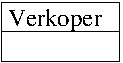
\includegraphics[width=2cm]{af1}
\end{center}\pause
\begin{itemize}
\item De verkoper wenst te beschikken over verschillende soorten gereedschap\ldots
\end{itemize}
\end{frame}


\begin{frame}
\frametitle{Het abstract factory pattern}
\begin{center}
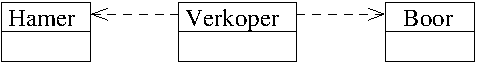
\includegraphics[width=7cm]{af2}
\end{center}
\begin{itemize}
\item De verkoper wenst van elk soort gereedschap een dure en goedkope variant te kunnen kopen\ldots
\end{itemize}
\end{frame}

\begin{frame}
\frametitle{Abstracties}
\begin{center}
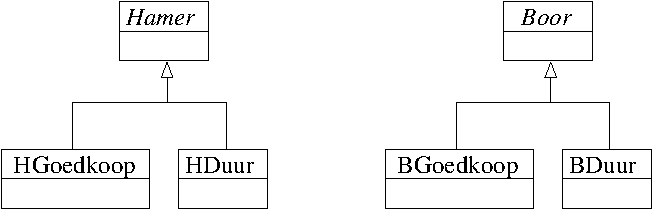
\includegraphics[width=10cm]{af3}
\end{center}
\end{frame}

\begin{frame}
\frametitle{Het abstract factory pattern}
\begin{center}
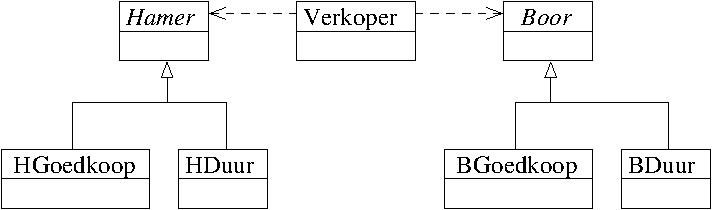
\includegraphics[width=10cm]{af4}
\end{center}
\begin{itemize}
\item De verkoper verkoopt \emph{een} boor en \emph{een} hamer\ldots
\end{itemize}
\end{frame}

\begin{frame}
\frametitle{Het abstract factory pattern}
De verkoper:
\begin{itemize}
\item bestelt gereedschap bij de fabriek
\item vertelt de fabriek slechts:
  \begin{itemize}
  \item welk gereedschap 
  \item wanneer en
  \item van welke soort
  \end{itemize}
\end{itemize}
Hoe die fabriek die spullen maakt en levert is de verantwoordelijkheid van de fabriek.
\end{frame}


\begin{frame}
\frametitle{Het abstract factory pattern}
\begin{center}
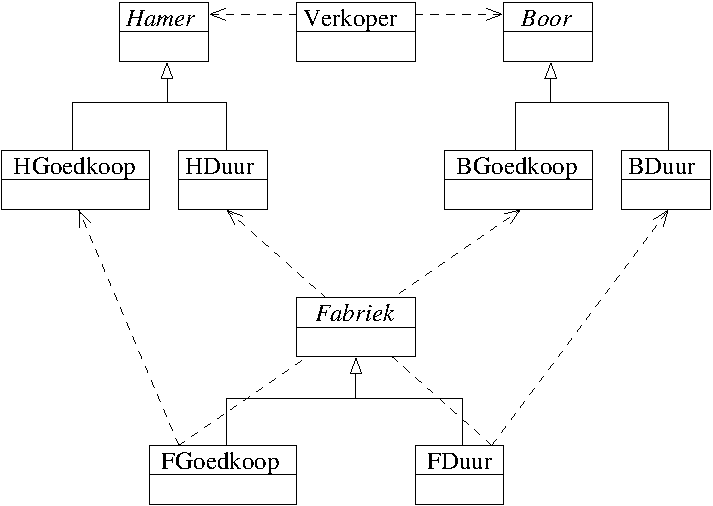
\includegraphics[width=9cm]{af5}
\end{center}
\end{frame}

\begin{frame}
\frametitle{Het abstract factory pattern}
\begin{itemize}
\item Naam: abstract factory pattern
\item Doel: omgaan met families van objecten
\item Hoe: creatie van objecten en \emph{hoe} dat gebeurt, scheiden van gebruik.
\item Gevolgen: nette boedelscheiding hoe en wat vragen $\rightarrow$ beter onderhoudbare en uitbreidbare code
\end{itemize}

\end{frame}


\begin{frame}
\frametitle{Het abstract factory pattern algemeen}
\begin{center}
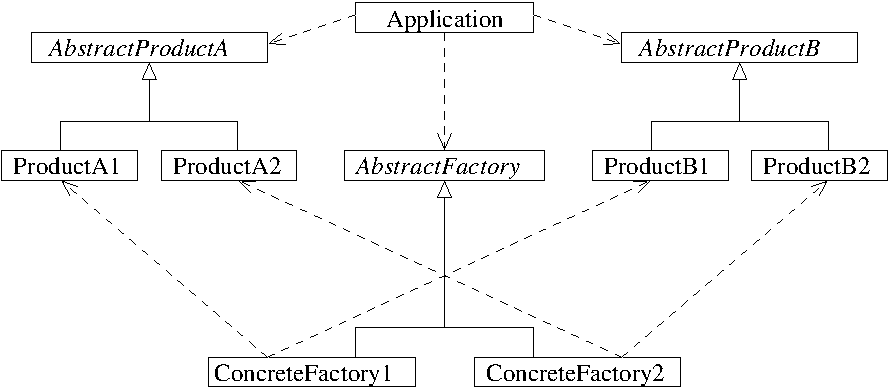
\includegraphics[width=10cm]{factory1}
\end{center}
\end{frame}

\end{document}